\section{树}
\subsection{树的概念和性质}
\subsubsection{树的概念}
\begin{definition}
\begin{enumerate}
	\item 不包含圈的图称为\colorbox{yellow}{\textcolor{red}{无圈图}},连通的无圈图称为\colorbox{yellow}{\textcolor{red}{树}},树通常用字母$T$表示.
	\item 一个无圈图称为\colorbox{yellow}{\textcolor{red}{森林}},树也是森林.
	\item 在一棵树中,度数为1的顶点称为树叶,度数大于1的顶点称为\textcolor{red}{分支点}.
	\item 平凡图称为\colorbox{yellow}{\textcolor{red}{平凡树}}.
\end{enumerate}
\begin{note}
	\begin{enumerate}
		\item \textcolor{red}{树和森林都是单图且都是偶图}.
		\item \textcolor{red}{非同构的4,5,6,7 阶树的棵数分别为2,3,6,11}.
	\end{enumerate}
	\begin{figure}[H]
	\small
	\centering 
	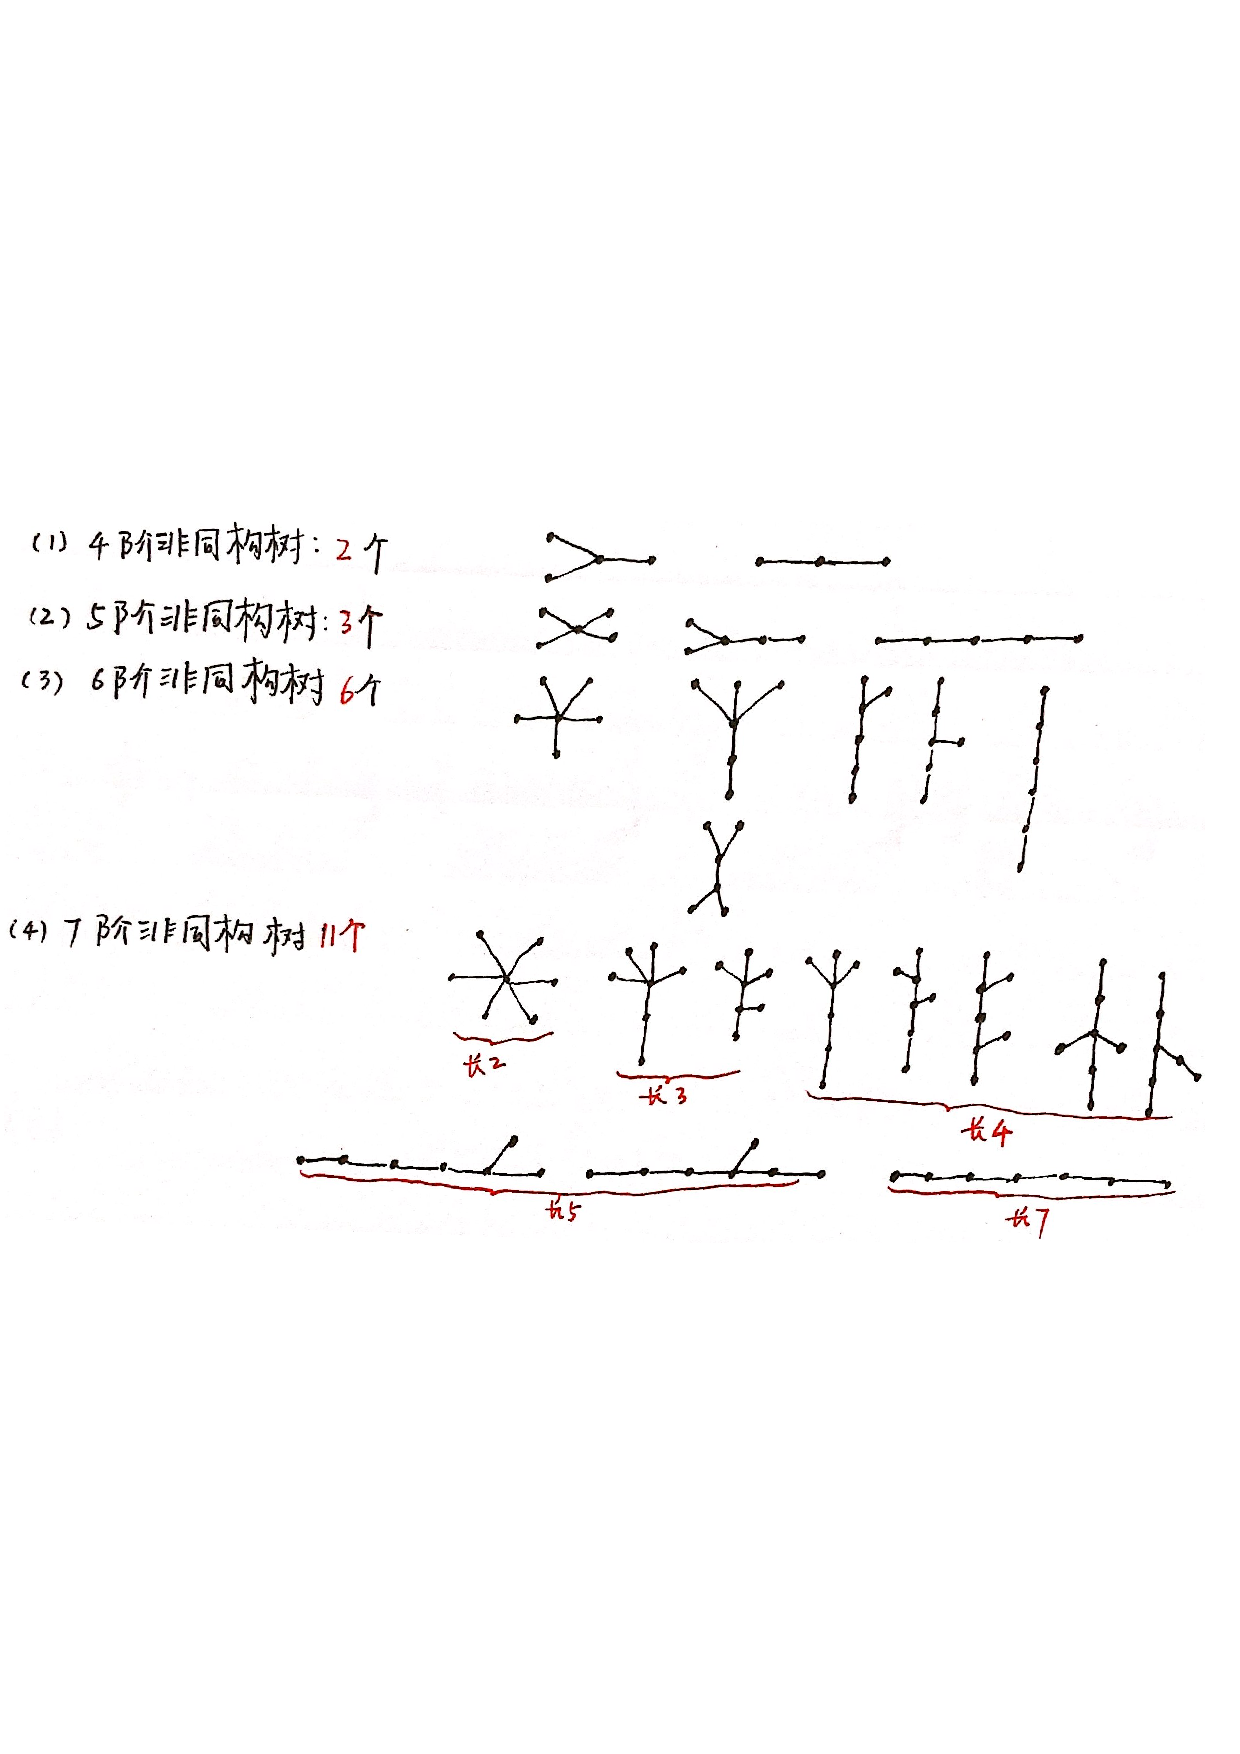
\includegraphics[scale=0.4]{image/CH2_tree.pdf}  
	%\caption{信息包结构} 
	\label{figff1ik}  
\end{figure}
\end{note}
	
\end{definition}

\subsubsection{树的性质}
\begin{theorem}
\label{hhh}
\textcolor{red}{每棵非平凡树至少有两片树叶}.
\end{theorem}
\begin{proof}
设$P=v_1v_2\cdots v_k$是非平凡树$T$中一条最长路,则$v_1$
与$v_k$在$T$中的邻接点只能有一个,否则,要么推出$P$
不是最长路,要么推出$T$中存在圈,这都是矛盾!
即说明$v_1$与$v_k$是树叶。
\end{proof}

\begin{example}
	$G$ 是树且 $\varDelta \geq k$,则 $G$ 至少有 $k$ 片叶子.
\end{example}
\begin{proof}
	若不然, 设 \( G \) 有 \( n \) 个顶点, \( m \) 条边且至多 \( k-1 \) 片叶子. 由于 \( \varDelta \geq k \), 于是由握手定理得
	\[
	2 m=\sum d(v) \geq 1 \cdot(k-1)+2 \cdot(n-k)+k \cdot 1=2 n-1>2 n-2
	\]
	所以, \( m>n-1 \), 与 \( G \) 是树矛盾!
\end{proof}

\begin{theorem}
	\label{kkkj}
	\textcolor{red}{图$G$是树当且仅当$G$中任意两点都被唯一的路连接.}
\end{theorem}
\begin{proof}
(1)必要性:图$G$是树,若不然,设$P1$与$P2$是连接$u$与$v$的两条不同的路。则由这两条路的全部或部分将构成一个圈,这与$G$是树相矛盾.

(2)充分性:首先,因$G$的任意两点均由唯一路相连,所以$G$是连通的。其次,若$G$中存在圈,则在圈中任取点$u$与$v$,可得到连接$u$与$v$的两条不同的路,与条件矛盾(定义,连通的无圈图即为树)。
\end{proof}
\begin{note}
$G$ 连通,删去任一边便不连通.
\end{note}



\begin{theorem}
设$T$是$(n, m)$树,则:
\[
\colorbox{yellow}{$ m=n-1$}
\]
\end{theorem}
\begin{proof}
对$n$作数学归纳.

当$n=1$时,等式显然成立;

设$n=k$时等式成立。考虑$n=k+1$的树$T$.
由定理\ref{hhh} $T$中至少有两片树叶,设$u$是$T$中树叶,考虑
$T1=T-u$,则$T1$为$k$阶树,于是$m(T1)=k-1$, 得$m(T)=k$.
\end{proof}


\begin{corollary}
\textcolor{red}{由$k$棵树组成的森林满足}:\colorbox{yellow}{$m=n-k$}.其中$n$为$G$的顶点数,$m$为$G$的边数.
\end{corollary}
\begin{proof}
设森林中每棵树的顶点数与边数分别是$n_i$和$m_i$($i=1,2,\cdots, k$),则由定理\ref{hhh}知,
\[
m_i = n_i -1, i = 1,2,\cdots, k
\]
因此
\[
\sum\limits_{i=1}^{k}m_i=\sum\limits_{i=1}^{k}(n_i -1)=n-k,
\]
即\[
m=n-k
\]
\end{proof}

\begin{theorem}
\textcolor{red}{每个$n$阶连通图的边数至少为$n-1$}.
\end{theorem}
\begin{proof}
   如果$n$阶连通图没有一度顶点,那么由握手定理
   有:
   \[
   m(G) = \dfrac{1}{2}\sum\limits_{v\in V(G)}d(v)\geq n
   \]
   
   如果$G$有一度顶点.对顶点数作数学归纳.
   
   当$n=1$时,结论显然成立.
   
   设当$n=k$时,结论成立,则
   
   当$n=k+1$时,设$u$是$G$的一度顶点,则$G-u$为具有$k$个顶
   点的连通图.
   
   若$G-u$有一度顶点,则由归纳假设,其边数至少$k-1$,于
   是$G$的边数至少有$k$条;
   
   若$G-u$没有一度顶点,则由握手定理:$m(G-u)=\dfrac{1}{2}\sum\limits_{v\in V(G-u)}d(v)\geq k$,所以$G$至少有$k+1$条边.
   
   而当$G$是树时,边数恰为$n-1$.所以$n$阶连通图$G$至少有$n-1$条边(\textcolor{red}{所以,树也被称为最小连通图.})
   
\end{proof}



\begin{theorem}
	\textcolor{red}{任意树T的两个不邻接顶点之间添加一条边后,
		可以得到唯一圈}.
\end{theorem}
\begin{proof}
设$u$与$v$是树$T$的任意两个不邻接顶点,由定理\ref{kkkj}
知:有唯一路$P$连接$u$与$v$.于是$P\cup\{uv\}$是 一个圈.

显然,由$P$的唯一性也就决定了$P\cup\{uv\}$ 的唯一性.
\end{proof}


\subsection{树的中心和形心}
\subsubsection{树的中心概念与性质}

\begin{enumerate}
	\item \textcolor{red}{图的顶点的离心率}:
	\[
	\colorbox{yellow}{$ e(v)=\mathrm{max} \{d(u,v)|u\in V(G)\}  $}
	\]
	\item \textcolor{red}{图的半径}:
	\[
	\colorbox{yellow}{$ r(G)=\mathrm{min} \{e(v)|v\in V(G)\}  $}
	\]
	\item \textcolor{red}{图的直径}: 最大离心率
	\item \textcolor{red}{图的中心点}: 离心率等于半径的点$e(v)= r(G)$
	\item \textcolor{red}{图的中心}: 中心点的集合
\end{enumerate}


\begin{theorem}
	每棵树的中心由一个点或两个相邻点组成.
\end{theorem}
%\begin{proof}
%	对树$T$的阶数$n$作归纳证明.
	
%	当$n=1$或$2$时,结论显然成立
	
%	设对$n<k(k\geq 3)$的树结论成立。设$T$是$k$阶树
	
%	容易知道:删掉$T$的所有叶,得到的树$T_1$的每个点的离心率
%	比它们在$T$中离心率减少1。又因$T$的叶不能是中心点,所以$T$
%	的中心点在$T_1$中。这样,若点$u$的离心率在$T$中最小,则在$T_1$中
%	依然最小,即说明$T$的中心点是$T_1$的中心点,反之亦然.
	
%	因为$T_1$的阶数$<k$,所以,由归纳假设,$T_1$的中心为一个点或两
%	个相邻点组成,即证明$T$的中心由一个点或两个相邻点组成.
%\end{proof}


\subsubsection{树的形心概念与性质}

\begin{definition}
	设$u$是树$T$的任意一个顶点,树$T$在顶点$u$的分支是指包含$u$
	作为一个叶点的极大子树,其\textcolor{red}{分支数}为顶点$u$的\colorbox{yellow}{\textcolor{red}{度数}};树$T$在
	$u$点的\textcolor{red}{ 分支中}边的最大数目称为点$u$的\colorbox{yellow}{\textcolor{red}{权}};树$T$中权值最小的
	点称为它的一个\colorbox{yellow}{\textcolor{red}{形心点}}。全体形心点的集合称为树$T$的形心.
\end{definition}
\begin{theorem}
	每棵树的形心由一个点或两个相邻点组成..
\end{theorem}

\subsection{生成树}
\subsubsection{生成树的概念和性质}

\begin{definition}
	图$G$的一个生成子图$T$如果是树,称它为$G$的一棵
	生成树;若$T$为森林,称它为$G$的一个生成森林.
	生成树的边称为\colorbox{yellow}{\textcolor{red}{树枝}},$G$中非生成树的边称为\colorbox{yellow}{\textcolor{red}{弦}}.
\end{definition}

\begin{theorem}
	每个连通图至少包含一棵生成树.
\end{theorem}
\begin{proof}
	如果连通图$G$是树,则其本身是一棵生成树;
	
	若连通图$G$中有圈$C$,则去掉$C$中一条边后得到的图仍
	然是连通的,这样不断去掉$G$中圈,最后得到一个$G$的
	无圈连通子图$T$,它为$G$的一棵生成树.
\end{proof}


\begin{corollary}
	\textcolor{red}{若$G$是$(n, m)$连通图,则$m\geq n-1$}.
\end{corollary}

\subsubsection{生成树的计数}

\noindent {\bfseries \textcolor{ecolor}{凯莱递推计数法:}}
\begin{definition}
	图$G$的边$e$称为\colorbox{yellow}{\textcolor{red}{被收缩}},是指删掉$e$后,把$e$的两
	个端点重合,如此得到的图记为$G\cdot e$.
\end{definition}

\begin{theorem}[Cayley]
	设$e$是$G$的一条边,则有:
	\[
	\colorbox{yellow}{\textcolor{red}{$\tau(G) = \tau(G-e) +\tau(G\cdot e) $}}
	\]
\end{theorem}
\begin{proof}
	$\tau(G-e)$是$G$不包含边$e$生成树的棵数. $G\cdot e$表示在$G$中删去$e$并重合其端点,则$\tau(G\cdot e)$是$G$包含边$e$生成树的棵数. 故$G$生成数的棵数$\tau(G) = \tau(G-e) +\tau(G\cdot e)$.
\end{proof}


\textcolor{red}{见PPT例题.}

\noindent {\bfseries \textcolor{ecolor}{矩阵树定理:}}

\begin{theorem}[矩阵树定理]
	设$G$是顶点集合为$V(G)=\{v_1,v_2,\cdots ,v_n\}$,
	的图,设$A=(a_{ij})$是$G$的邻接矩阵,$C=(c_{ij})$是$n$阶方阵,其中:
	\[
	\colorbox{yellow}{$
		c_{ij}=\left\{\begin{array}{cc}
			d(v_i)&i=j \\
			-a_{ij}& i \ne j
		\end{array}\right.
		$}
	\]
	则$G$的生成树棵数为$C$的任意一个\textcolor{red}{代数余子式}的值.
\end{theorem}
\begin{note}
	矩阵$C$又称为图的拉普拉斯矩阵,即
	\[
	\colorbox{yellow}{$ C=D(G)-A(G)$}
	\]其中,$D(G)$是图的度对角矩阵,即主对角元为对应顶
	点度数,其余元素为0.
\end{note}

\begin{theorem}
	\colorbox{yellow}{$\tau(K_n) = n^{n-2}\quad \tau(K_{m,n})=n^{m-1}m^{n-1}$}
\end{theorem}

\begin{proof}
	\textcolor{red}{使用矩阵树定理证明}
	
	写出拉普拉斯矩阵$C$,然后计算某行某列的余子式即可得证.
\end{proof}

\subsubsection{回路系统简介}

\begin{definition}
	设$T$是连通图$G$的一棵生成树,把属于$G$但不属于$T$
	的边称为$G$关于$T$的\colorbox{yellow}{\textcolor{red}{连枝}},$T$中的边称为$G$关于$T$的\colorbox{yellow}{\textcolor{red}{树枝}}
\end{definition}

\begin{definition}
	设$T$是连通图$G$的一棵生成树,由$G$的对应于$T$\textcolor{red}{一条连
		枝}与$T$中树枝构成的唯一圈$C$,称为$G$关于$T$的一个基本圈或
	基本回路.若$G$是$(n, m)$连通图,把$G$对应于$T$的\colorbox{yellow}{\textcolor{red}{$m-n+1$}}个基
	本回路称为$G$对应于$T$的基本回路组,记为$C_f$ .
\end{definition}

\begin{theorem}
	连通图$G$的任一回路均可表示成若干个基本回路的\colorbox{yellow}{\textcolor{red}{对称差}}
\end{theorem}

\subsection{最小生成树}
\begin{definition}
	在连通边赋权图$G$中求一棵总权值最小的生成树.该生成树称为\textcolor{red}{最小生成树或最小代价树}.
\end{definition}

\subsubsection{克鲁斯克尔算法}
\noindent 算法步骤:
\begin{enumerate}
	\item 选择边$e_1$,使得其权值最小;
	\item 若已经选定边$e_1, e_2,\cdots, e_k$, 则从$E-\{e_1, e_2,\cdots, e_k\}$中选择边$e_{k+1}$,使得:
	\begin{itemize}
		\item $G[e_1, e_2,\cdots, e_{k+1}]$为无圈图;
		\item $e_{k+1}$的权值$w(e_{k+1})$尽可能小.
	\end{itemize}
	\item 当(2)不能进行时,停止.
	
\end{enumerate}
\begin{note}
	由克鲁斯克尔算法得到的任何生成树一定是最小
	生成树.
\end{note}

\subsubsection{管梅谷的破圈法}

破圈法求最小生成树的求解过程是:从赋权图G的任
意圈开始,去掉该圈中权值最大的一条边,称为破圈。
不断破圈,直到G中没有圈为止,最后剩下的G的子图
为G的最小生成树.
\subsubsection{Prim算法}


\noindent 算法步骤:
\begin{enumerate}
	\item 对于连通赋权图$G$的任意一个顶点$u$,选择与点$u$关
	联的且权值最小的边作为最小生成树的第一条边$e_1$;
	\item 在接下来的边$G[e_2, e_3,\cdots, e_{m}]$ ,在与一条已经选取的边\textcolor{red}{只
		有一个公共端点}的的所有边中,\textcolor{red}{选取权值最小}的边.直到找到最小生成树.	
\end{enumerate}


\subsubsection{根树简介}
\begin{definition}
	\begin{enumerate}
	\item 对于\textcolor{red}{有向树}$T$的顶点$v$来说,存在\textcolor{red}{入度}和\textcolor{red}{出度}.
	\item 一棵非平凡的有向树$T$,\textcolor{red}{如果恰有一个顶点的入度为0,而其余所有顶点的入度为1,这样的的有向树称为\colorbox{yellow}{根树}}. 其中入度为0的点称为\colorbox{yellow}{\textcolor{red}{树根}},出度为0的点称为\colorbox{yellow}{\textcolor{red}{树叶}},入度为1,出度大于1的点称为\colorbox{yellow}{\textcolor{red}{内点}}. 又将内点和树根统称为\colorbox{yellow}{\textcolor{red}{分支点}}
	\item 对于根树$T$,顶点$v$到树根的距离称为点$v$的层数;
	所有顶点中的层数的最大者称为根树$T$的\colorbox{yellow}{\textcolor{red}{树高}}.
	\item 对于根树$T$,若规定了每层顶点的访问次序,这
	样的根树称为\colorbox{yellow}{\textcolor{red}{有序树}}.
	\item 对于根树$T$,若每个分支点至多$m$个儿子,称该
	根树为\colorbox{yellow}{\textcolor{red}{$m$元根树}};若每个分支点恰有$m$个儿子,称它为
	\colorbox{yellow}{\textcolor{red}{完全$m$元根树}}.
	\begin{note}
		\textcolor{red}{高度为$h$的完全二元树最多有$h+1$片树叶}.
	\end{note}
\end{enumerate}
\end{definition}


\noindent 对于完全m元树T,有如下性质:
\begin{theorem}
	在完全$m$元树$T$中,若树叶数为$t$ , 分支点数为$i$ , 则:
	\[
	\colorbox{yellow}{$(m-1)i= t-1 $}
	\]
\end{theorem}
\begin{proof}
	由树的性质得:
	$m(T) = n-1 = t+i -1$
	
	由握手定理得:$2m(T)=t+m+(i-1)(m+1)$
	
	联立得结论.
\end{proof}


\noindent 有序树转化为二元树:\textcolor{red}{长子兄弟法}.

\noindent 二元树的遍历: \textcolor{red}{先序遍历、中序遍历、后序遍历}.


\subsubsection{最优二元树}
\begin{definition}
设 \( T \) 是一棵有 \( t \) 片树叶的二元树, 若对 \( T \) 的所有 \( t \) 片树叶赋以权值 (实 数) \( w_{1}, w_{2}, \cdots, w_{t} \), 则称 \( T \) 为带权二元树; 若带有权 \( w_{i} \) 的树叶的层数为 \( l\left(w_{i}\right) \), 则称
\[
W(T)=\sum_{i=1}^{t} w_{i} l\left(w_{i}\right)
\]为 $T$ 的权;$W(T)$ 最小的二元树称为最优树.
\end{definition}

 \textcolor{red}{哈夫曼算法}.
\begin{example}
	求带权为:7、8、9、12、16的最优树.
	\begin{figure}[H]
		\small
		\centering 
		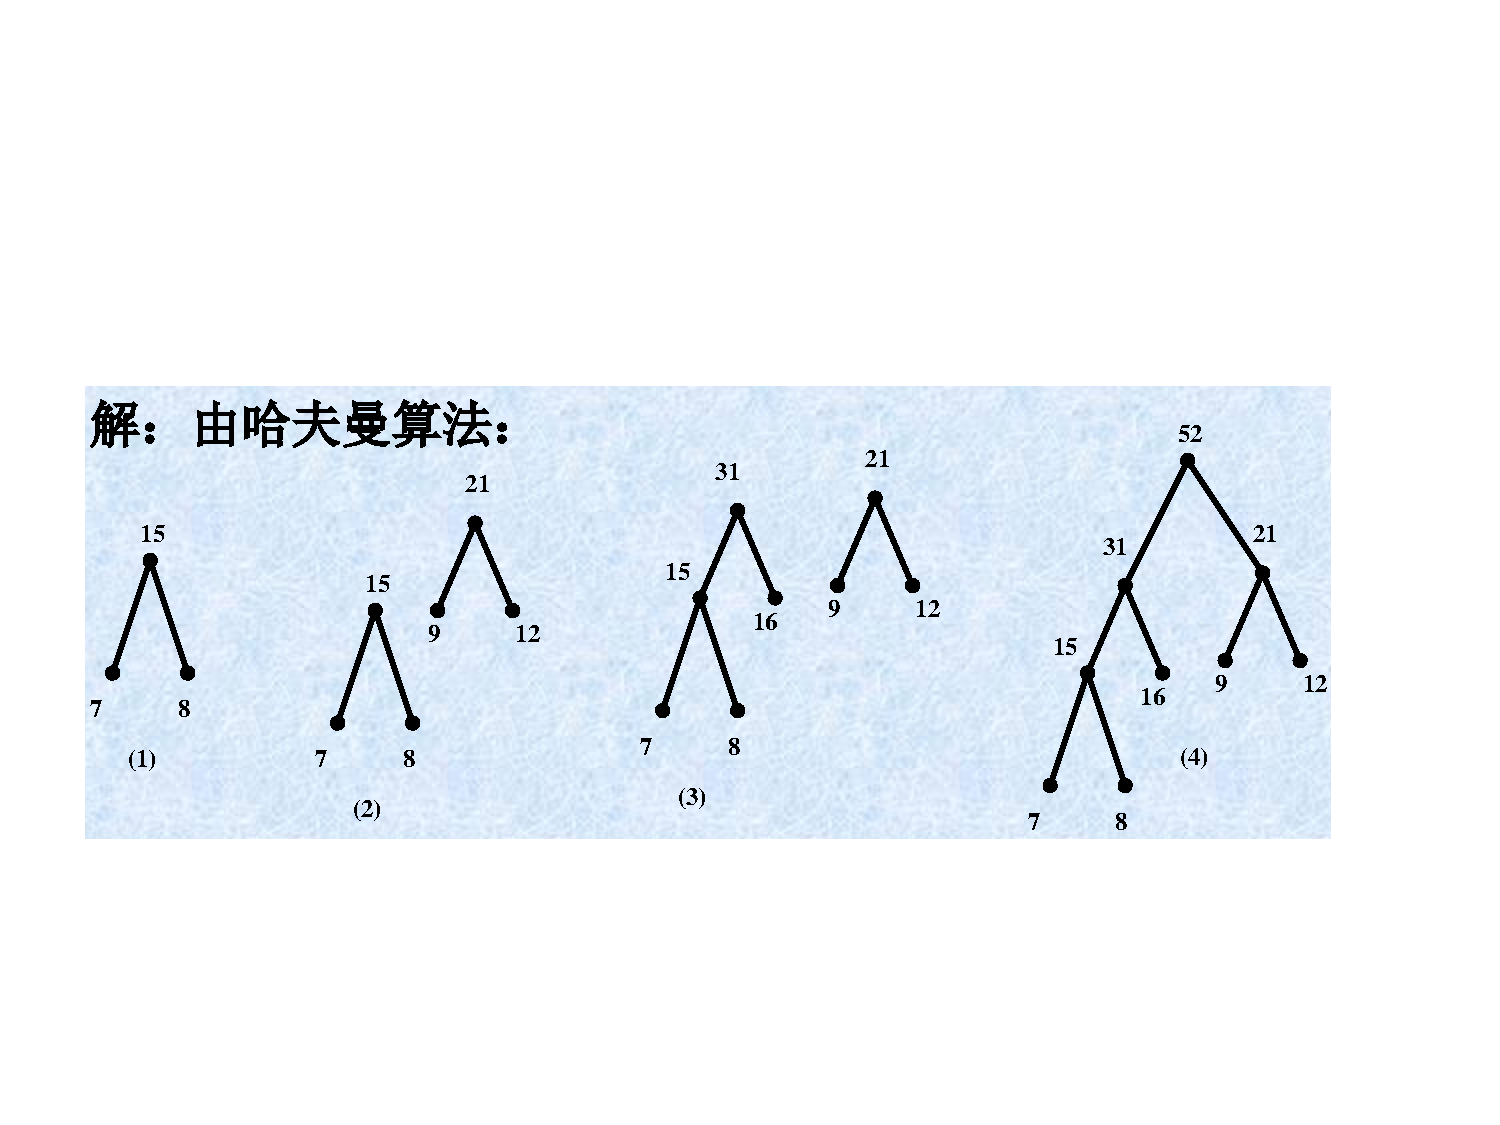
\includegraphics[scale=0.65]{image/CH2_hufman.pdf}  
		%\caption{信息包结构} 
		\label{figkff1ik}  
	\end{figure}

设求得的最优二元树为 $T$,则

$W(T)=(7+8)\times 3+(16+9+12)\times 2=119$
\end{example}







